\documentclass[dvipsnames,crop=true]{standalone}
\usepackage{tikz}
\usepackage{currfile}
\usetikzlibrary{calc,external,3d}
\begin{document}

  \tikzsetnextfilename{policies}

  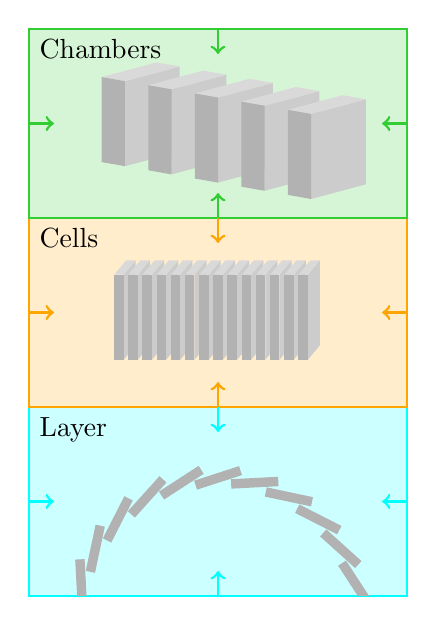
\begin{tikzpicture}[scale=0.6,line width=1pt]


    \begin{scope}[fill opacity=0.2]
        \filldraw[Cyan] (0,0) rectangle ++(8,4);
        \filldraw[Orange] (0,4) rectangle ++(8,4);
        \filldraw[LimeGreen] (0,8) rectangle ++(8,4);
    \end{scope}

    \foreach \c/\y\l in {Cyan/0/Layer,Orange/4/Cells,LimeGreen/8/Chambers} {
        \begin{scope}[draw=\c,shift={(0,\y)}]
            \node[anchor=north west] at (0,4) {\l};
            \draw[->] (0,2) --++(15pt,0);
            \draw[->] (8,2) --++(-15pt,0);
            \draw[->] (4,0) --++(0,15pt);
            \draw[->] (4,4) --++(0,-15pt);
        \end{scope}
    }

    \begin{scope}[shift={(4,-0.5)}]
        \clip (-4,0.5) rectangle ++(8,4);
        \foreach \d in {0,15,...,180} {
            \begin{scope}[rotate=\d]
                \begin{scope}[shift={(3,0)}]
                    \begin{scope}[rotate=18]
                        \fill[black!30] (-0.1,-0.5) rectangle ++(0.2,1);
                    \end{scope}
                \end{scope}
            \end{scope}
        }
    \end{scope}

    \begin{scope}[shift={(4,5)}]
        \foreach \z in {-2,-1.7,...,2} {
            \begin{scope}[scale=1,x={(50:0.2cm)},y={(90:0.9cm)},z={(0:1cm)}]
                \begin{scope}[canvas is xy plane at z={\z}]
                    \fill[black!20] (0,0) rectangle ++(2,2);
                \end{scope}
                \begin{scope}[canvas is xz plane at y={2}]
                    \fill[black!15] (0,\z) rectangle ++(2,-0.2);
                \end{scope}
                \begin{scope}[canvas is yz plane at x={0}]
                    \fill[black!30] (0,\z) rectangle ++(2,-0.2);
                \end{scope}
            \end{scope}
        }
        % \foreach \x in {-2,-1,...,2} {
        %     \begin{scope}[shift={(\x,-1.3)},scale=1,x={(30:0.5cm)},y={(90:0.9cm)},z={(-10:1cm)}]
        %         \begin{scope}[canvas is xy plane at z={0}]
        %             \fill[black!20] (0,0) rectangle ++(2,2);
        %         \end{scope}
        %         \begin{scope}[canvas is xz plane at y={2}]
        %             \fill[black!15] (0,0) rectangle ++(2,-0.5);
        %         \end{scope}
        %         \begin{scope}[canvas is yz plane at x={0}]
        %             \fill[black!30] (0,0) rectangle ++(2,-0.5);
        %         \end{scope}
        %     \end{scope}
        % }
    \end{scope}

    \begin{scope}[shift={(4,8.75)}]
        % \foreach \x in {-2,-1.5,...,2} {
        %     \begin{scope}[shift={(\x,0)}]
        %         \begin{scope}[rotate=80]
        %             \fill[black!30] (0,0) rectangle ++(2,0.3);
        %         \end{scope}
        %     \end{scope}
        % }

        \foreach \z in {-2,-1,...,2} {
            \begin{scope}[scale=1,x={(15:0.6cm)},y={(90:0.9cm)},z={(-10:1cm)}]
                \begin{scope}[canvas is xy plane at z={\z}]
                    \fill[black!20] (0,0) rectangle ++(2,2);
                \end{scope}
                \begin{scope}[canvas is xz plane at y={2}]
                    \fill[black!15] (0,\z) rectangle ++(2,-0.5);
                \end{scope}
                \begin{scope}[canvas is yz plane at x={0}]
                    \fill[black!30] (0,\z) rectangle ++(2,-0.5);
                \end{scope}
            \end{scope}
        }

    \end{scope}


  \begin{scope}[scale=1,x={(30:0.5cm)},y={(90:0.9cm)},z={(-10:1cm)}]
  \end{scope}

  \end{tikzpicture}

\end{document}